\section{Structure and function of heart valves}
    
    Heart valves are complex multi-layered structures that prevent backflow by opening and closing depending on the direction of flow. There are four valves in the heart, consisting of two atrioventricular preventing backflow between the atriums and ventricles, the mitral (MV) and tricuspid valves (TV), and two semilunar preventing backflows from the aorta and to the vena cava, the aortic (AV) and pulmonary valves (PV) (Fig. \ref{fig:heartdiagram}). The coordinated movement of the four heart valves enables them to maintain unidirectional blood flow during the cardiac cycle. When healthy, heart valves are incredibly resilient, opening and closing approximately 3 - 4 billion times throughout an average life-span \cite{sacks_biomechanics_2009}. The pressure changes during the cardiac cycle expose the heart valves to constant changes in forces and hemodynamics. This physiological demand is especially harsh on the mitral and aortic valves, needing to withstand average pressures of 80mmHg for the aortic and 120mmHg for the mitral valve to sustain circulation throughout the rest of the body. The biomechanical properties of heart valves must be able to withstand and function efficiently in this complex mechanical environment. Thus, the heart valve leaflets develop and maintain an intricate, highly organized, and multi-scale connective tissue system that allows them to do so \cite{tao_heart_2012}. 

%-------------------	begin FIGURE 	-------------------%
\begin{figure}
\centering
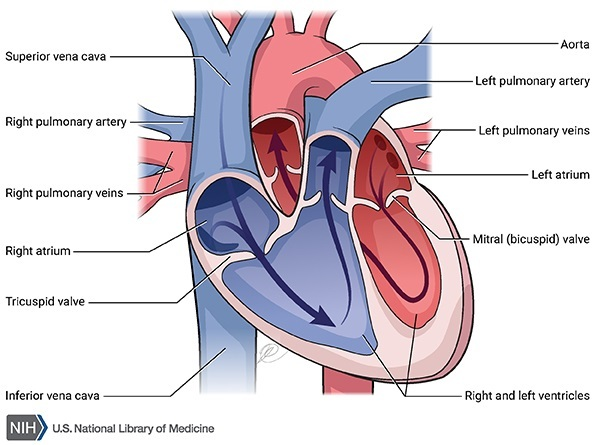
\includegraphics[width=5.0in]{Images/chapter1/heartdiagram.jpeg}
\caption{Artist rendition of the human heart depicting the location of the four heart valves and major vessels (obtained from U.S. National Library of Science website)}
\label{fig:heartdiagram}
\end{figure}
%-------------------	 end FIGURE 	-------------------%

\subsection{Multi-scale structure of heart valves}

    To fully understand the functional properties of heart valves, multi-scale approaches are needed (Fig. \ref{fig:multiscalevalve}) \cite{salma_heart_2016}. This complex hierarchical structure is what lends to seamless heart valve performance under highly dynamic loading conditions. Heart valves have evolved to have multi-layered leaflet structures. The aortic valve, for example, consists of three histologically distinct layers, whereas the mitral valve has four (Fig. \ref{fig:valvelayers}). The fibrosa layer, which is located on the ventricular side of atrioventricular valves and the atrial side of semilunar valves, is composed of circumferentially aligned collagen fibers that provide the leaflets with the necessary tensile strength to open and transmit forces during coaptation while closed. The spongiosa layer is situated adjacent to the fibrosa and though it contains some collagen, its main constituents are the hydrophilic glycosaminoglycans and proteoglycans, which give the valve its compressive properties and allow it to absorb high forces during coaptation. The ventricularis and atrialis are the layers that are adjacent to blood flow in atrioventricular valvesand semilunar valves, respectively. These layers are rich in radially oriented elastin fibers and facilitate the closure movement by extending the valve leaflet as it opens and recoils when it closes. The annulus and chordae tendineae of the atrioventricular valves and the connection between the leaflets and the surrounding myocardium in the semilunar valves provide additional support. 
    


%-------------------	begin FIGURE 	-------------------%
\begin{figure}
\centering
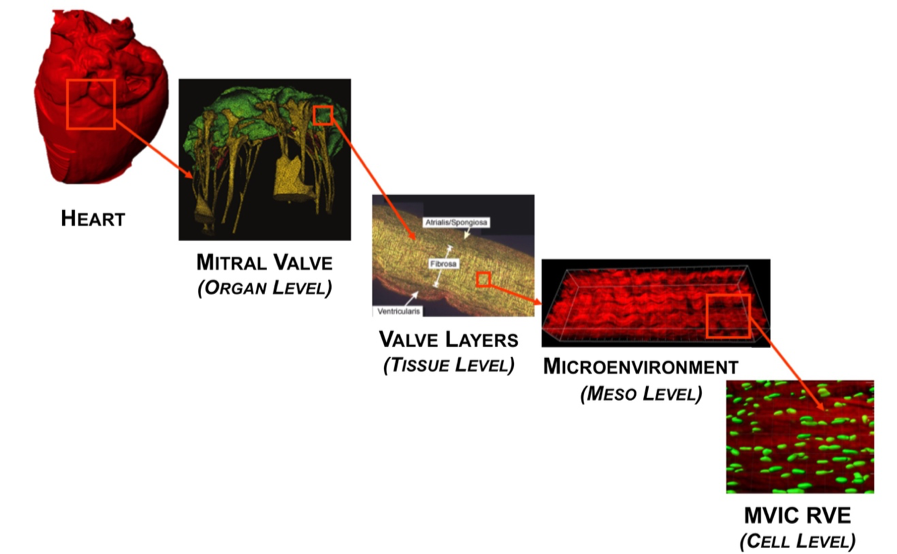
\includegraphics[width=\textwidth]{Images/chapter1/multiscalevalve.png}
\caption{The multiscale nature of heart valve biomechanics: a representation of the mitral valve at the organ-, tissue-, and cell-levels. At the tissue-level: a circumferentially oriented cross-section of the mitral valve anterior leaflet stained with Movat pentachrome, which colors collagen yellow, elastic fibers black, and hydrated PGs and GAGs blue. At the cell-level: a transmission electron micrograph of a mitral VIC from the fibrosa layer. (Adapted from \cite{salma_heart_2016})}
\label{fig:multiscalevalve}
\end{figure}
%-------------------	 end FIGURE 	-------------------%


%-------------------	begin FIGURE 	-------------------%
\begin{figure}
\centering
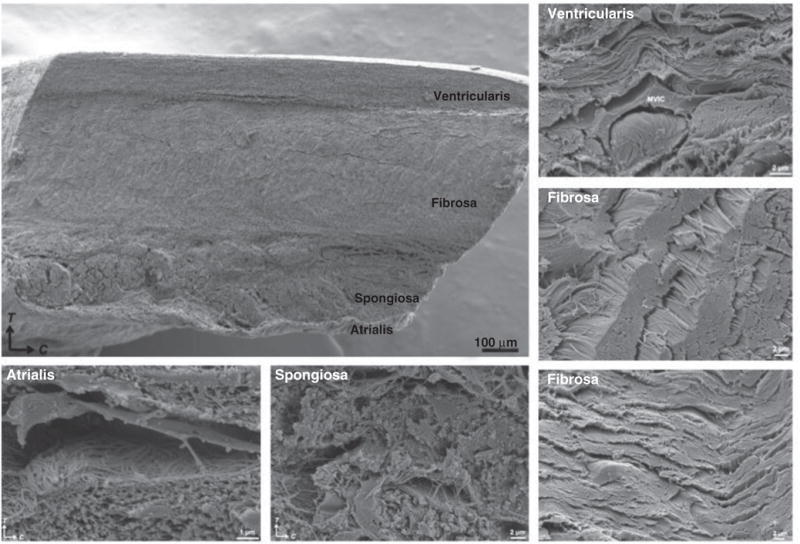
\includegraphics[width=\textwidth]{Images/chapter1/valvelayers.jpg}
\caption{Scanning electron micrograph of the multilayered microenvironment of the MV anterior leaflet. Individual micrographs of each layer are also presented: elastin-rich ventricularis and atrialis, highly collagenous fibrosa, and proteoglycan-rich spongiosa. The collagen fibrils and elastic fibers closely surround the interstitial cells and highlight the long cellular extensions. In the fibrosa, collagen fibrils are aligned in the circumferential direction of the leaflet, which is responsible for the observed anisotropy in leaflet mechanical behavior. (T: transmural, C: circumferential). (Adapted from \cite{salma_heart_2016}.)}
\label{fig:valvelayers}
\end{figure}
%-------------------	 end FIGURE 	-------------------%
   




    The collagen dense fibrosa layer is the predominant stress-bearing layer. Collagen fibers have low torsional and flexural stiffness but can withstand high tensile forces. As such, fiber orientation can be used as an identifier for the material axes of the tissue, or in other words the directions in which the tissue is able to withstand the greatest tensile stresses. To measure the orientation distribution of the collagen fibers, small angle light scattering (SALS) is a popular choice \cite{sacks_small_1997}. In this technique, a beam of laser, 500-600 nm in wavelength, is passed through a tissue specimen and is then scattered. The spatial intensity distribution of the resulting scattered light depends on the orientation of the collagen fibers (which is at a similar length scale as the light particles), which can in turn be used to obtain structural information of the tissue. As an example, Sacks et al. used SALS to quantify the changes that occur in AV leaflet structure with increasing transvalvular pressure (TVP) \cite{sacks_aortic_1998}.  Fresh porcine AVs were fixed at TVPs ranging from 0 to 90 mmHg and imaged using small angle light scattering (SALS). Overall, increasing TVP induced the greatest changes in fiber alignment between 0 and 1 mmHg, and past 4 mmHg there was no detectable improvement in fiber alignment (Fig. \ref{c1:fig:salsaortic}b-d). 
    
    
%-------------------	begin FIGURE 	-------------------%
\begin{figure}
\centering
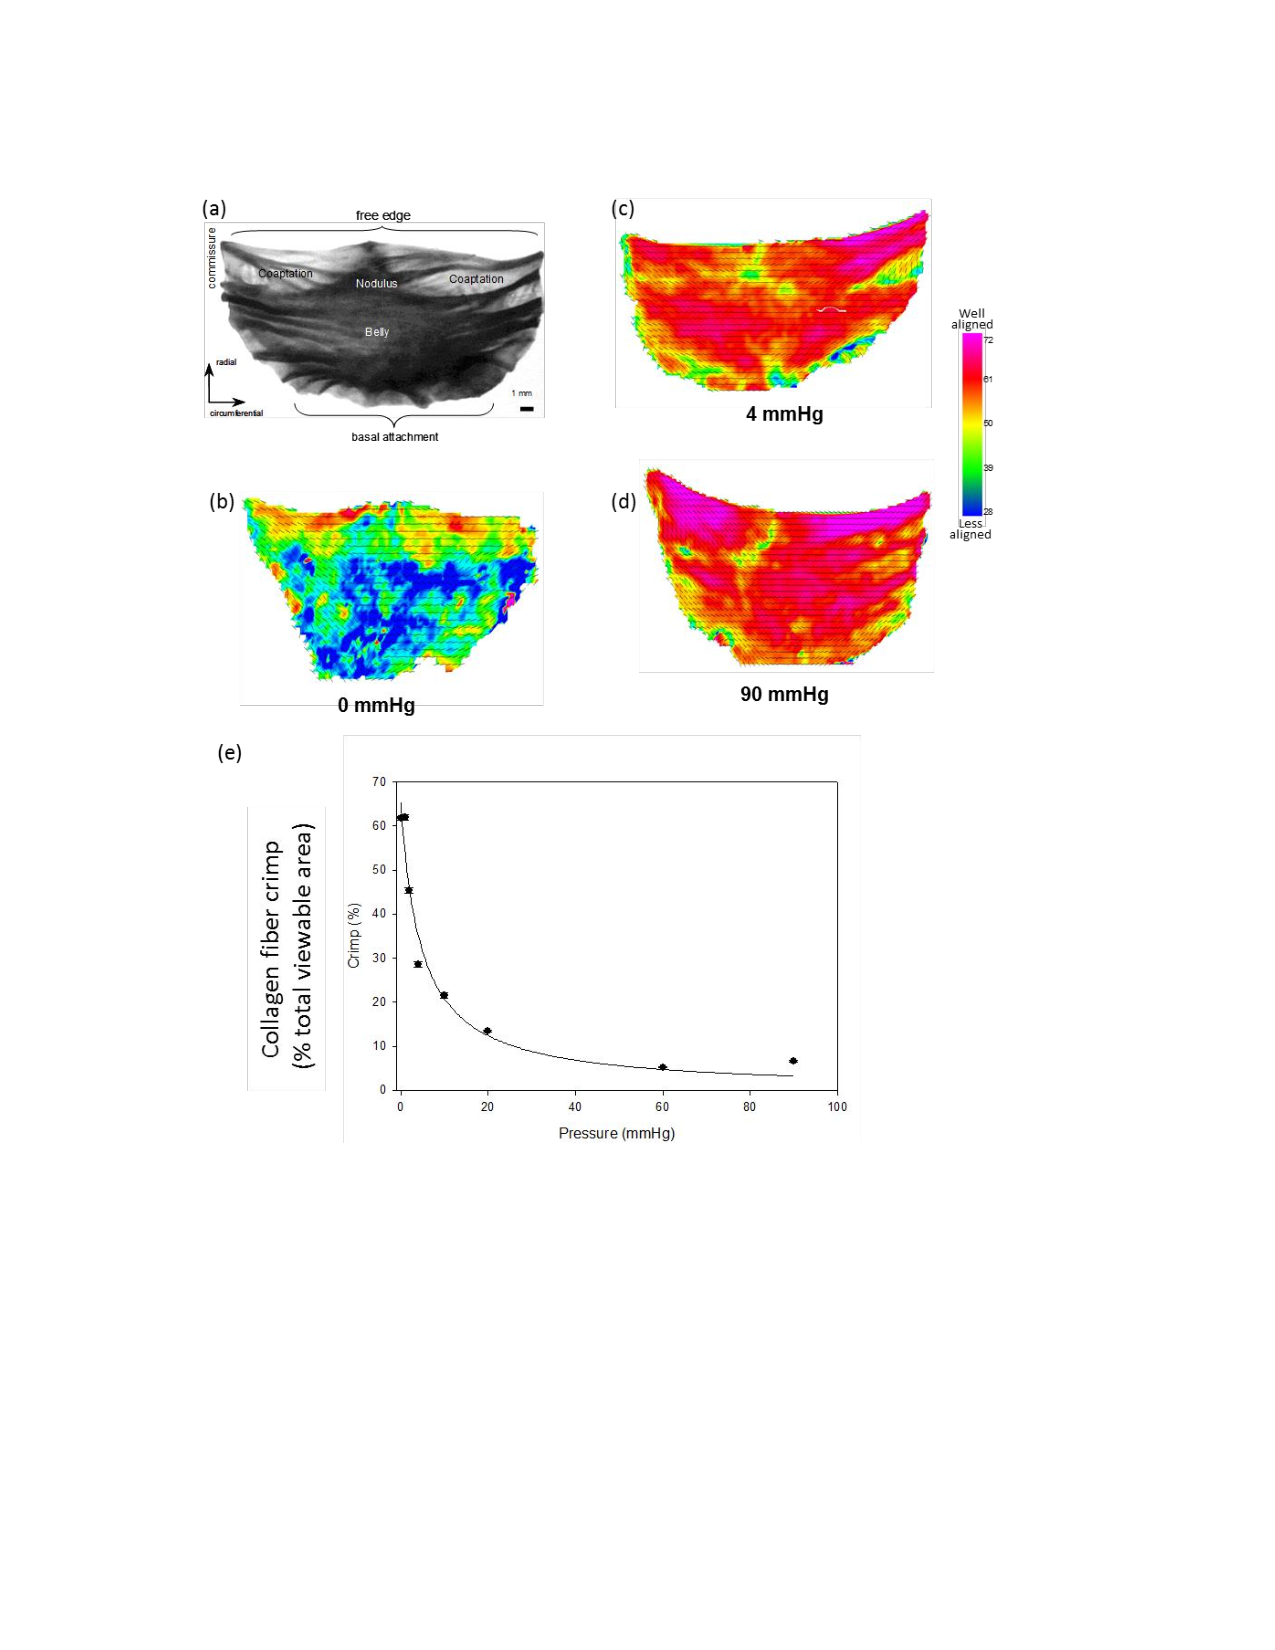
\includegraphics[width=5.5in]{Images/chapter1/salsaortic.pdf}
\caption{(a) Diagram of the AV cusp highlighting the belly, commissures, nodulus, and regions of coaptation. Small angle light scattering results with the orientation index at (b) 0mmHg, (c) 4mmHg, and (d) 90mmHg transvalvular pressure. No further changes in fiber alignment were observed past 4mmHg. These results are consistent with histological-based data that quantifies the percent area of tissue displaying collagen fiber crimp (e). (Adapted from Sacks et al. \cite{sacks_aortic_1998})}
\label{c1:fig:salsaortic}
\end{figure}
%-------------------	 end FIGURE 	-------------------%

    
    The other most important structural information about collagen fibers is the amount to which the collagen fibers are crimped. As collagen fibers have low torsional and flexural stiffness, they bear minimal stresses before they are fully straightened. Thus, the stretch needed to straighten these collagen fibers will determine the compliance or extensibility at the tissue-level. One example for the attempt to quantification of collagen fiber crimp is the methods of Hilbert et al. \cite{hilbert_optical_1986, hilbert_porcine_1990}. They quantified the amount of collagen fiber crimp in the native pulmonary and aortic HVs by identifying the cross-sectional regions that displayed observable crimp \cite{joyce_functional_2009}. It was found that at 0 mmHg, approximately 60\% of the AV transverse cross-sectional area was occupied by crimp structure (Fig. \ref{c1:fig:salsaortic}e). As the TVP increased, the percent crimp decreased rapidly until 20 mmHg, with minimal decreases in percent crimp thereafter. For the AV, much of the observed change in collagen structure is due to the finely tuned straightening of the collagen fibers, which must occur at the right strain level and at the right rate to facilitate coaptation without allowing excessive tissue deformations that could lead to regurgitation. The unique structure of the commissure region, which approximately corresponds to the coaptation region, highlights the adaptive structure of HVs. Instead of undergoing TVP differences, the coaptation region is loaded in a uniaxial-like manner due to tethering forces generated at the attachment of the commissures to the aortic root. Unlike the biaxially loaded belly regions of the valve, the uniaxial loading of the commissures makes them more highly aligned, similar to tendon. Fiber uncrimping with stress occurs very rapidly for this highly aligned fiber network, as demonstrated by the short transition region from low to high stiffness. The highly aligned nature of the commissure region at unloaded state and the more rapid realignment with TVP in the 10 commissure regions are consistent with the pre-transition strain level behavior of tendon- like materials. 